\setAuthor{}
\setRound{lõppvoor}
\setYear{2020}
\setNumber{G 1}
\setDifficulty{1}
\setTopic{TODO}

\prob{Klaaskera}
Taskulambiga, millest väljuva valgusvihu läbimõõt on $d$, valgustatakse suurt
klaasist kera läbimõõduga $D$. Milline peaks olema klaasi murdumisnäitaja, et
valgusvihk kera keskpunkti suunates koonduks klaaskera pinnal? Eeldada, et
valgusvihu diameeter on tunduvalt väikesem kera läbimõõdust ($d\ll D$) ning et
taskulambist väljuv valgusvihk on paralleelne.

\emph{Vihje:} Väikeste nurkade korral $\sin \alpha \approx \alpha$, kui $\alpha$
on radiaanides.


\hint

\solu
Mööda optilist peatelge liikuv kiir ei murdu ning liigub otse läbi kera. Seega koonduvad kõik kiired kera tagumise poole ja optilise peatelje lõikumiskohta. Uurime nüüd üht valguskiirt, mis asub vihu tsentrist eemal. Selle konkreetse valguskiire jaoks võib lähendada probleemi kahedimensionaalseks. Joonistame kiire käigu, märgime nurgad. Langemisnurk olgu $\alpha$ ning murdumisnurk $\beta$, kusjuures need on omavahel seotud Snelli seadusega: $n_{õ}\sin\alpha=n_{k}\sin\beta$. Sarnaste kolmnurkade tõttu $\angle AOB$ on samuti $\alpha$. Kolmnurk $AFO$ on võrdhaarne (haaradeks kera raadiused) ning seega $\angle AFO$ on $\beta$. Ühelt poolt (kolmnurga sisenurkade summa on $180^\circ$) $\angle AOF=180-2\beta$, teisalt (kõrvunurkade summa on $180^\circ$) $\angle AOF=180^\circ-\alpha$, seega $\alpha=2\beta$. Võttes, et $n_{õ}=1$ ning tehes väikeste nurkade lähenduse $\sin x \approx x$, saame:
$$n_{õ}\sin\alpha=n_{k}\sin\beta \Rightarrow \sin2\beta=n_{k}\sin\beta \Rightarrow n_k = \frac{\sin2\beta}{\sin\beta}\approx\frac{2\beta}{\beta}=2.$$
\begin{figure}[htbp!]
\centering
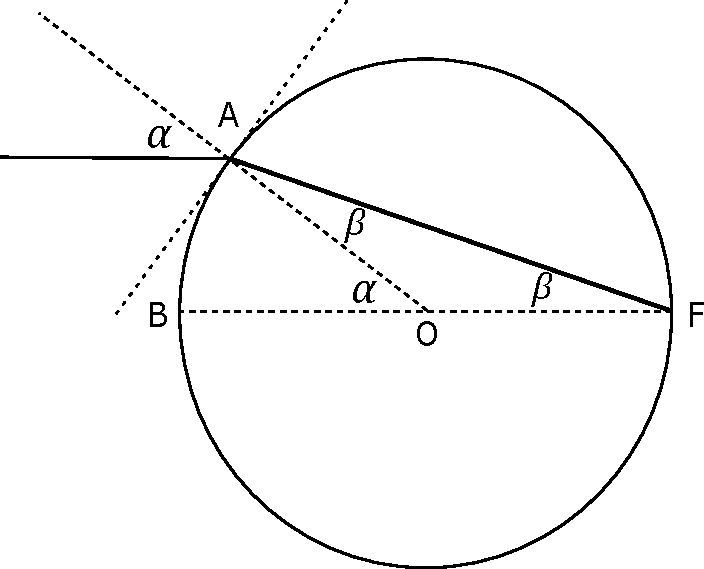
\includegraphics[width=0.6\textwidth]{2020-v3g-01-yl.pdf}
\end{figure}
\probend